\documentclass[12pt]{article}

\usepackage[a4paper,margin=1in]{geometry}
\usepackage{setspace}
\onehalfspacing

\usepackage{amsmath,amssymb,amsthm}
\usepackage{graphicx}
\usepackage{float}
\usepackage{caption}
\usepackage{subcaption}
\usepackage{enumitem}

\title{ECON 5345 Homework 11 Report}
\author{Harlly Zhou}
\date{\today}

\begin{document}

\maketitle

Starting from the initial guess $V_0(a) = \vec{0}$, VFI result is shown below in Figure \ref{fig:1}.
\begin{figure}[htbp]
    \centering
    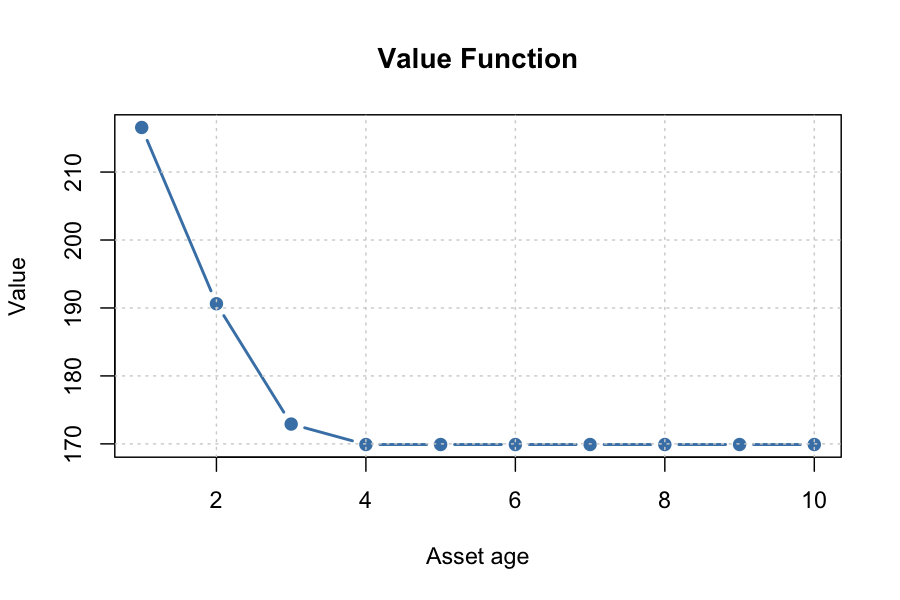
\includegraphics[width=0.6\textwidth]{hw11_output/hw11_value_function.png}
    \caption{Value function}
    \label{fig:1}
\end{figure}

We can see that the optimal replacement policy is to replace the asset when it is 4 years old. Hence, the path of state variable is in Figure \ref{fig:2}.
\begin{figure}[htbp]
    \centering
    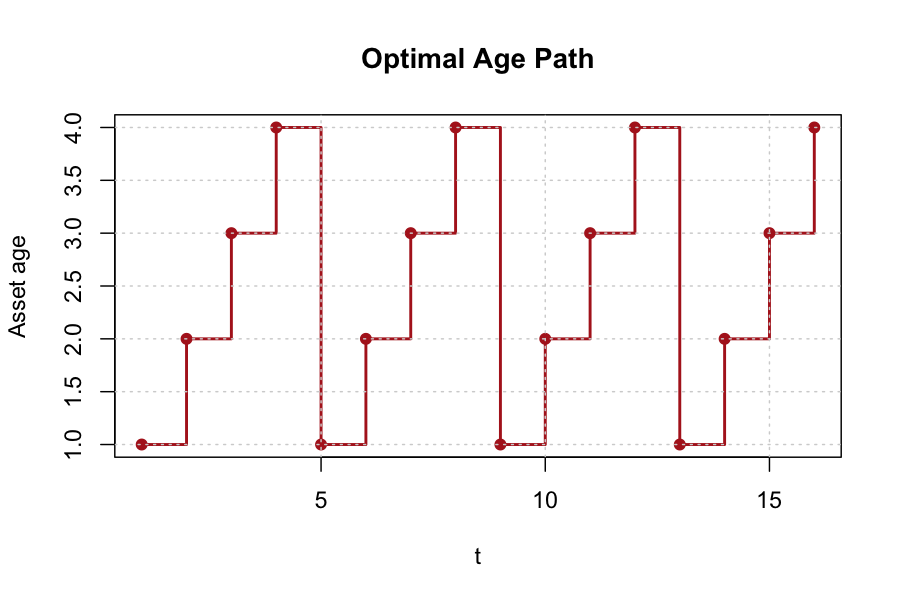
\includegraphics[width=0.6\textwidth]{hw11_output/hw11_optimal_age_path.png}
    \caption{Optimal age path}
    \label{fig:2}
\end{figure}

To prove that 4 is really the cutoff age, we can solve the problem analytically. Guess that the cutoff age is $a^* > 1$. Then
\begin{align*}
    V(a) \equiv V^* := p(0) - c + \beta V(1) = 0.9 V(1) - 25, \forall a \geq a^*.
\end{align*}
Note that 
\begin{align*}
    V(a) = \sum_{j=0}^{a^*-a-1} p(a+j) + \beta^{a^*-a} V^*
\end{align*}
To verify that $a^*=4$, what we need to show is that $p(4) + 0.9 V^* \leq V^*$ and $p(3) + 0.9 V^* > V^*$.. 
Note that $p(1) = 45$, $p(2) = 35$, $p(3) = 20$, $p(4) = 0$, so we have
\begin{align*}
    p(4) + 0.9 V^* = 0 + 0.9 V^* \leq V^*.
\end{align*}
By backward induction formula, we have $V(1) = 92.7 + 0.729 V^*$. Substituting this into $V^* = 0.9V(1) - 25$, we get $V^* = 169.9040$. Hence $20 + 0.9V^* > V^*$.

Therefore, $a^*=4$ is actually the cutoff.

\end{document}